\newpage
\subsection{Projection Imaging}

In this module we begin to explore imaging with the MR scanner by introducing spatial encoding along one dimension. We do this by adding a single gradient to the spin echo spectroscopy sequence used in previous modules. Playing this gradient during readout enables spatial discrimination along the gradient dimension. The resulting data can then be reconstructed into a 1D image by means of Fourier transformation, with the other two orthogonal dimensions being projected. Alternatively, additional projections may be acquired to resolve a higher-dimensional image, e.g. like the back-projection algorithm does for x-ray computed tomography (CT).

Figure \ref{fig:grad-axes} shows the OCRA naming convention for the gradient axes. The $x$ axis points to the right, the $y$ axis points up, and the $z$ axis points forward. This agrees with the conventional MR nomenclature \emph{in the lab frame}. However keep in mind that relative to the bore axis the $y$ and $z$ axes are actually swapped compared with convention. It's all a matter of perspective, isn't it?

\begin{wrapfigure}{r}{6cm}
    \centering
    \vspace{-10mm}
    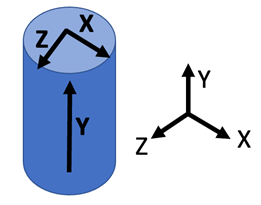
\includegraphics[width=6cm]{grad-axes}
    \caption{\label{fig:grad-axes} OCRA naming convention for gradient axes with sample bore in blue.}
    \vspace{-10mm}
\end{wrapfigure}

\subsubsection{Water Phantom}
Use a water-only phantom for this portion of the experiment. You will measure projections along the $x$, $y$, and $z$ axes.

\begin{enumerate}
    \item   Navigate to the main menu. Click \textbf{Projections} and select \textbf{Spin Echo (On Axis)}.
    \item   Open \textbf{Parameters}. Under \emph{General}, set TE to 10 ms, TR to 2000ms, Sampling Time to 6 ms. Under \emph{Imaging}, set Image Resolution to 64 and FOV to 30 mm. Under \emph{Projections}, select X, Y, and Z to iterate through each gradient axis one at a time.
    \item   Click \textbf{Acquire}, then \textbf{Data Process}.
\end{enumerate}

Observe the resulting plots of frequency spectra in $x$, $y$, and $z$. Adjust the frequency range to better visualize the profile. The 2D image plot is XZ plane and is reconstructed from only these three basic projections, hence the result is very crude.

\noindent{}\color{red}
Save a screenshot of the spectral plots and comment on their appearance.
\color{black}

\subsubsection{Mystery (?) Phantom}
Now you will repeat the above experiment to probe a mystery phantom. The mystery phantom is labelled with a question mark. It contains one or more water-filled holes oriented along $y$. Your task is to use projection imaging to deduce the number of water-filled holes in this phantom. Hint: try rotating the phantom to capture different projection angles.

\noindent{}\color{red}
How many holes are in the mystery phantom? Explain your reasoning and include screenshots to support your conclusion. 
\color{black}